%%%%%%%%%%%%%%%%%%%%%%%%%%%%%%%%%%%%%%%%%%%%%%%%%%%%%%%%%%%%
%%  This Beamer template was created by Cameron Bracken.
%%  Anyone can freely use or modify it for any purpose
%%  without attribution.
%%
%%  Last Modified: January 9, 2009
%%

\documentclass[xcolor=x11names,compress]{beamer}

%% General document %%%%%%%%%%%%%%%%%%%%%%%%%%%%%%%%%%
\usepackage{graphicx}
\usepackage{tikz}
\usetikzlibrary{decorations.fractals}
%%%%%%%%%%%%%%%%%%%%%%%%%%%%%%%%%%%%%%%%%%%%%%%%%%%%%%


%% Beamer Layout %%%%%%%%%%%%%%%%%%%%%%%%%%%%%%%%%%
\useoutertheme[subsection=false,shadow]{miniframes}
\useinnertheme{default}
\usefonttheme{serif}
\usepackage{palatino}
\usepackage{graphicx}
\usepackage{multicol}
\usepackage{amsmath}
\usepackage{epic,eepic,epsfig}
\usepackage{amssymb}
\usepackage{amstext}
\usetikzlibrary{shapes.geometric}

\usepackage{tikz}
\usepackage{mathtools}
\usetikzlibrary{arrows}
\usetikzlibrary{positioning}

\setbeamerfont{title like}{shape=\scshape}
\setbeamerfont{frametitle}{shape=\scshape}

\setbeamercolor*{lower separation line head}{bg=gray}%DeepSkyBlue4} 
\setbeamercolor*{normal text}{fg=black,bg=white} 
\setbeamercolor*{alerted text}{fg=red} 
\setbeamercolor*{example text}{fg=black} 
\setbeamercolor*{structure}{fg=black} 
 
\setbeamercolor*{palette tertiary}{fg=black,bg=black!10} 
\setbeamercolor*{palette quaternary}{fg=black,bg=black!10} 

\renewcommand{\(}{\begin{columns}}
\renewcommand{\)}{\end{columns}}
\newcommand{\<}[1]{\begin{column}{#1}}
\renewcommand{\>}{\end{column}}
%%%%%%%%%%%%%%%%%%%%%%%%%%%%%%%%%%%%%%%%%%%%%%%%%%

\begin{document}

%%%%%%%%%%%%%%%%%%%%%%%%%%%%%%%%%%%%%%%%%%%%%%%%%%%%%%
%%%%%%%%%%%%%%%%%%%%%%%%%%%%%%%%%%%%%%%%%%%%%%%%%%%%%%
\section{\scshape Introduction}
\begin{frame}
\title{How many oblivious robots can explore a line}
\author{
	Paola Flocchini  David Ilcinkas  Andrzej Pels  Nicola Santoro\\
	\vspace{24pt} 
	\includegraphics[width=1\textwidth,right]{robot1.jpg}
}
\titlepage
\end{frame}

%%%%%%%%%%%%%%%%%%%%%%%%%%%%%%%%%%%%%%%%%%%%%%%%%%%%%%
%%%%%%%%%%%%%%%%%%%%%%%%%%%%%%%%%%%%%%%%%%%%%%%%%%%%%%
% \begin{frame}{Introduction}
% \begin{multicols}{2}
% \tableofcontents
% \includegraphics[width=.4\textwidth,right]{robot1.jpg}
% \end{multicols}
% \end{frame}

%%%%%%%%%%%%%%%%%%%%%%%%%%%%%%%%%%%%%%%%%%%%%%%%%%%%%%
%%%%%%%%%%%%%%%%%%%%%%%%%%%%%%%%%%%%%%%%%%%%%%%%%%%%%%
\section{\scshape Model}
\subsection{frame 1}
\begin{frame}{Definition} %%% MODEL 1 %%%
\begin{tabular}{rl}
  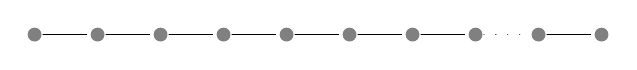
\begin{tikzpicture}[scale=0.8,->,>=stealth',shorten >=1pt,auto,node distance=3cm,
    thick,main node/.style={circle,draw,font=\footnotesize}, small node/.style={circle,font=\footnotesize,inner sep=0pt,minimum size=5pt}]   
    \begin{scope}     
%     \node[inner sep=0pt] (robot) at (4,5)
%     {\includegraphics[width=.02\textwidth,right]{robot1.jpg} };
      \node[small node,fill=gray] (a) at (1,5) {};
      \node[small node,fill=gray] (b) at (2,5) {};
      \node[small node,fill=gray] (c) at (3,5) {};
      \node[small node,fill=gray] (d) at (4,5) {};
      \node[small node,fill=gray] (e) at (5,5) {};    
      \node[small node,fill=gray] (f) at (6,5) {};
      \node[small node,fill=gray] (g) at (7,5) {};
      \node[small node,fill=gray] (h) at (8,5) {};
      \node[small node,fill=gray] (i) at (9,5) {};
      \node[small node,fill=gray] (j) at (10,5) {}; 
      \path[-,line width=0.3pt] (a) edge (b);
      \path[-,line width=0.3pt] (b) edge (c);
      \path[-,line width=0.3pt] (c) edge (d);
      \path[-,line width=0.3pt] (d) edge (e);
      \path[-,line width=0.3pt] (e) edge (f);
      \path[-,line width=0.3pt] (f) edge (g);
      \path[-,line width=0.3pt] (g) edge (h);
      \path[-,line width=0.3pt, loosely dotted] (h) edge (i);
      \path[-,line width=0.3pt] (i) edge (j);
    \end{scope}
  \end{tikzpicture} 
  & $n$ nodes\\ 
    &  \\
    &  \\
    &  \\
    &  \\
    &  \\
\end{tabular}
\end{frame}

\begin{frame}{Definition} %%% MODEL 1 %%%
\begin{tabular}{rl}
  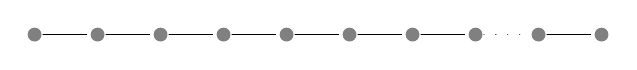
\begin{tikzpicture}[scale=0.8,->,>=stealth',shorten >=1pt,auto,node distance=3cm,
    thick,main node/.style={circle,draw,font=\footnotesize}, small node/.style={circle,font=\footnotesize,inner sep=0pt,minimum size=5pt}]   
    \begin{scope}     
%     \node[inner sep=0pt] (robot) at (4,5)
%     {\includegraphics[width=.02\textwidth,right]{robot1.jpg} };
      \node[small node,fill=gray] (a) at (1,5) {};
      \node[small node,fill=gray] (b) at (2,5) {};
      \node[small node,fill=gray] (c) at (3,5) {};
      \node[small node,fill=gray] (d) at (4,5) {};
      \node[small node,fill=gray] (e) at (5,5) {};    
      \node[small node,fill=gray] (f) at (6,5) {};
      \node[small node,fill=gray] (g) at (7,5) {};
      \node[small node,fill=gray] (h) at (8,5) {};
      \node[small node,fill=gray] (i) at (9,5) {};
      \node[small node,fill=gray] (j) at (10,5) {}; 
      \path[-,line width=0.3pt] (a) edge (b);
      \path[-,line width=0.3pt] (b) edge (c);
      \path[-,line width=0.3pt] (c) edge (d);
      \path[-,line width=0.3pt] (d) edge (e);
      \path[-,line width=0.3pt] (e) edge (f);
      \path[-,line width=0.3pt] (f) edge (g);
      \path[-,line width=0.3pt] (g) edge (h);
      \path[-,line width=0.3pt, loosely dotted] (h) edge (i);
      \path[-,line width=0.3pt] (i) edge (j);
    \end{scope}
  \end{tikzpicture} 
  & $n$ nodes\\ 
    &  \\
    &  \\
    &  \\
    &  \\
    &  \\
\end{tabular}
\end{frame}

\begin{frame}{Definition} %%% MODEL 2 %%%
\begin{tabular}{rl}
  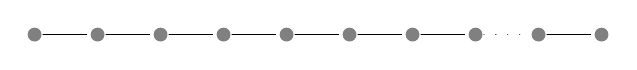
\begin{tikzpicture}[scale=0.8,->,>=stealth',shorten >=1pt,auto,node distance=3cm,
    thick,main node/.style={circle,draw,font=\footnotesize}, small node/.style={circle,font=\footnotesize,inner sep=0pt,minimum size=5pt}]   
    \begin{scope}     
%     \node[inner sep=0pt] (robot) at (4,5)
%     {\includegraphics[width=.02\textwidth,right]{robot1.jpg} };
      \node[small node,fill=gray] (a) at (1,5) {};
      \node[small node,fill=gray] (b) at (2,5) {};
      \node[small node,fill=gray] (c) at (3,5) {};
      \node[small node,fill=gray] (d) at (4,5) {};
      \node[small node,fill=gray] (e) at (5,5) {};    
      \node[small node,fill=gray] (f) at (6,5) {};
      \node[small node,fill=gray] (g) at (7,5) {};
      \node[small node,fill=gray] (h) at (8,5) {};
      \node[small node,fill=gray] (i) at (9,5) {};
      \node[small node,fill=gray] (j) at (10,5) {}; 
      \path[-,line width=0.3pt] (a) edge (b);
      \path[-,line width=0.3pt] (b) edge (c);
      \path[-,line width=0.3pt] (c) edge (d);
      \path[-,line width=0.3pt] (d) edge (e);
      \path[-,line width=0.3pt] (e) edge (f);
      \path[-,line width=0.3pt] (f) edge (g);
      \path[-,line width=0.3pt] (g) edge (h);
      \path[-,line width=0.3pt, loosely dotted] (h) edge (i);
      \path[-,line width=0.3pt] (i) edge (j);
    \end{scope}
  \end{tikzpicture} 
  & $n$ nodes\\ 
      &  \\
  \includegraphics[width=.05\textwidth,right]{robot1.jpg} 
  \includegraphics[width=.05\textwidth,right]{robot1.jpg} 
  \includegraphics[width=.05\textwidth,right]{robot1.jpg}  
  \includegraphics[width=.05\textwidth,right]{robot1.jpg} 
  & $k$ robots\\
    &  \\
    &  \\
    &  \\
\end{tabular}
\end{frame}

\begin{frame}{Definition} %%% MODEL 3 %%%
\begin{tabular}{rl}
  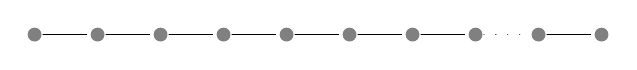
\begin{tikzpicture}[scale=0.8,->,>=stealth',shorten >=1pt,auto,node distance=3cm,
    thick,main node/.style={circle,draw,font=\footnotesize}, small node/.style={circle,font=\footnotesize,inner sep=0pt,minimum size=5pt}]   
    \begin{scope}     
%     \node[inner sep=0pt] (robot) at (4,5)
%     {\includegraphics[width=.02\textwidth,right]{robot1.jpg} };
      \node[small node,fill=gray] (a) at (1,5) {};
      \node[small node,fill=gray] (b) at (2,5) {};
      \node[small node,fill=gray] (c) at (3,5) {};
      \node[small node,fill=gray] (d) at (4,5) {};
      \node[small node,fill=gray] (e) at (5,5) {};    
      \node[small node,fill=gray] (f) at (6,5) {};
      \node[small node,fill=gray] (g) at (7,5) {};
      \node[small node,fill=gray] (h) at (8,5) {};
      \node[small node,fill=gray] (i) at (9,5) {};
      \node[small node,fill=gray] (j) at (10,5) {}; 
      \path[-,line width=0.3pt] (a) edge (b);
      \path[-,line width=0.3pt] (b) edge (c);
      \path[-,line width=0.3pt] (c) edge (d);
      \path[-,line width=0.3pt] (d) edge (e);
      \path[-,line width=0.3pt] (e) edge (f);
      \path[-,line width=0.3pt] (f) edge (g);
      \path[-,line width=0.3pt] (g) edge (h);
      \path[-,line width=0.3pt, loosely dotted] (h) edge (i);
      \path[-,line width=0.3pt] (i) edge (j);
    \end{scope}
  \end{tikzpicture} 
  & $n$ nodes\\ 
      &  \\
  \includegraphics[width=.05\textwidth,right]{robot1.jpg} 
  \includegraphics[width=.05\textwidth,right]{robot1.jpg} 
  \includegraphics[width=.05\textwidth,right]{robot1.jpg}  
  \includegraphics[width=.05\textwidth,right]{robot1.jpg} 
  & $k$ robots\\
    &  \\
        &  \\
    \begin{tikzpicture}[scale=0.8,->,>=stealth',shorten >=1pt,auto,node distance=3cm,
    thick,main node/.style={circle,draw,font=\footnotesize}, small node/.style={circle,font=\footnotesize,inner sep=0pt,minimum size=5pt}]   
    \begin{scope}     
%     \node[inner sep=0pt] (robot) at (4,5)
%     {\includegraphics[width=.02\textwidth,right]{robot1.jpg} };
      \node[small node,fill=gray] (a) at (1,5) {};
      \node[inner sep=0pt]  (b) at (2,5) {\includegraphics[width=.03\textwidth,right]{robot1.jpg}};
      \node[small node,fill=gray] (c) at (3,5) {};
      \node[inner sep=0pt]  (d) at (4,5) {\includegraphics[width=.03\textwidth,right]{robot1.jpg}};
      \node[inner sep=0pt]  (e) at (5,5) {\includegraphics[width=.03\textwidth,right]{robot1.jpg}};    
      \node[small node,fill=gray] (f) at (6,5) {};
      \node[inner sep=0pt]  (g) at (7,5) {\includegraphics[width=.03\textwidth,right]{robot1.jpg}};
      \node[small node,fill=gray] (h) at (8,5) {};
      \node[small node,fill=gray] (i) at (9,5) {};
      \node[small node,fill=gray] (j) at (10,5) {}; 
      
%       \node[inner sep=0pt]   at (2,5.5) {\includegraphics[width=.03\textwidth,right]{robot1.jpg}};
%       \node[inner sep=0pt]   at (5,5.5) {\includegraphics[width=.03\textwidth,right]{robot1.jpg}};
%       \node[inner sep=0pt]   at (5,6) {\includegraphics[width=.03\textwidth,right]{robot1.jpg}};
      \path[-,line width=0.3pt] (a) edge (b);
      \path[-,line width=0.3pt] (b) edge (c);
      \path[-,line width=0.3pt] (c) edge (d);
      \path[-,line width=0.3pt] (d) edge (e);
      \path[-,line width=0.3pt] (e) edge (f);
      \path[-,line width=0.3pt] (f) edge (g);
      \path[-,line width=0.3pt] (g) edge (h);
      \path[-,line width=0.3pt, loosely dotted] (h) edge (i);
      \path[-,line width=0.3pt] (i) edge (j);
    \end{scope}
  \end{tikzpicture}
  & \\
\end{tabular}
\end{frame}

\begin{frame}{Definition} %%% MODEL 4 %%%
\begin{tabular}{rl}
  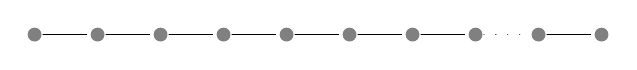
\begin{tikzpicture}[scale=0.8,->,>=stealth',shorten >=1pt,auto,node distance=3cm,
    thick,main node/.style={circle,draw,font=\footnotesize}, small node/.style={circle,font=\footnotesize,inner sep=0pt,minimum size=5pt}]   
    \begin{scope}     
%     \node[inner sep=0pt] (robot) at (4,5)
%     {\includegraphics[width=.02\textwidth,right]{robot1.jpg} };
      \node[small node,fill=gray] (a) at (1,5) {};
      \node[small node,fill=gray] (b) at (2,5) {};
      \node[small node,fill=gray] (c) at (3,5) {};
      \node[small node,fill=gray] (d) at (4,5) {};
      \node[small node,fill=gray] (e) at (5,5) {};    
      \node[small node,fill=gray] (f) at (6,5) {};
      \node[small node,fill=gray] (g) at (7,5) {};
      \node[small node,fill=gray] (h) at (8,5) {};
      \node[small node,fill=gray] (i) at (9,5) {};
      \node[small node,fill=gray] (j) at (10,5) {}; 
      \path[-,line width=0.3pt] (a) edge (b);
      \path[-,line width=0.3pt] (b) edge (c);
      \path[-,line width=0.3pt] (c) edge (d);
      \path[-,line width=0.3pt] (d) edge (e);
      \path[-,line width=0.3pt] (e) edge (f);
      \path[-,line width=0.3pt] (f) edge (g);
      \path[-,line width=0.3pt] (g) edge (h);
      \path[-,line width=0.3pt, loosely dotted] (h) edge (i);
      \path[-,line width=0.3pt] (i) edge (j);
    \end{scope}
  \end{tikzpicture} 
  & $n$ nodes\\ 
      &  \\
  \includegraphics[width=.05\textwidth,right]{robot1.jpg} 
  \includegraphics[width=.05\textwidth,right]{robot1.jpg} 
  \includegraphics[width=.05\textwidth,right]{robot1.jpg}  
  \includegraphics[width=.05\textwidth,right]{robot1.jpg} 
  & $k$ robots\\
    &  \\
        &  \\
    \begin{tikzpicture}[scale=0.8,->,>=stealth',shorten >=1pt,auto,node distance=3cm,
    thick,main node/.style={circle,draw,font=\footnotesize}, small node/.style={circle,font=\footnotesize,inner sep=0pt,minimum size=5pt}]   
    \begin{scope}     
     \node[inner sep=0pt] (robot) at (4,5)
     {\includegraphics[width=.02\textwidth,right]{robot1.jpg} };
      \node[small node,fill=gray] (a) at (1,5) {};
      \node[inner sep=0pt]  (b) at (2,5) {\includegraphics[width=.03\textwidth,right]{robot1.jpg}};
      \node[small node,fill=gray] (c) at (3,5) {};
      \node[inner sep=0pt]  (d) at (4,5) {\includegraphics[width=.03\textwidth,right]{robot1.jpg}};
      \node[inner sep=0pt]  (e) at (5,5) {\includegraphics[width=.03\textwidth,right]{robot1.jpg}};    
      \node[small node,fill=gray] (f) at (6,5) {};
      \node[inner sep=0pt]  (g) at (7,5) {\includegraphics[width=.03\textwidth,right]{robot1.jpg}};
      \node[small node,fill=gray] (h) at (8,5) {};
      \node[small node,fill=gray] (i) at (9,5) {};
      \node[small node,fill=gray] (j) at (10,5) {}; 
      
       \node[inner sep=0pt]   at (2,5.5) {\includegraphics[width=.03\textwidth,right]{robot1.jpg}};
       \node[inner sep=0pt]   at (5,5.5) {\includegraphics[width=.03\textwidth,right]{robot1.jpg}};
       \node[inner sep=0pt]   at (5,6) {\includegraphics[width=.03\textwidth,right]{robot1.jpg}};
      \path[-,line width=0.3pt] (a) edge (b);
      \path[-,line width=0.3pt] (b) edge (c);
      \path[-,line width=0.3pt] (c) edge (d);
      \path[-,line width=0.3pt] (d) edge (e);
      \path[-,line width=0.3pt] (e) edge (f);
      \path[-,line width=0.3pt] (f) edge (g);
      \path[-,line width=0.3pt] (g) edge (h);
      \path[-,line width=0.3pt, loosely dotted] (h) edge (i);
      \path[-,line width=0.3pt] (i) edge (j);
    \end{scope}
  \end{tikzpicture}
  & \\
\end{tabular}
\end{frame}

\begin{frame}{Look}
%\resizebox{<horizontal size>}{<vertical size>}{%
    \begin{tikzpicture}[scale=0.8,->,>=stealth',shorten >=1pt,auto,node distance=3cm,
    thick,main node/.style={circle,draw,font=\footnotesize}, small node/.style={circle,font=\footnotesize,inner sep=0pt,minimum size=5pt}]   

    \begin{scope}%[xshift=10cm]
      \node[small node,fill=gray] (b) at (2,5) {};
      \node[inner sep=0pt]  (c) at (4,5) {\includegraphics[width=.03\textwidth,right]{robot1.jpg}};
      \node[inner sep=0pt]  (d) at (6,5) {\includegraphics[width=.03\textwidth,right]{robot1.jpg}};
      \node[small node,fill=gray] (e) at (8,5) {};    
      \node[inner sep=0pt]  (f) at (10,5) {\includegraphics[width=.03\textwidth,right]{robot1.jpg}};
      \node[inner sep=0pt] at (10,5.5) {\includegraphics[width=.03\textwidth,right]{robot1.jpg}};
      \node[small node,fill=gray] (i) at (12,5) {};
      \node[small node,fill=gray] (j) at (14,5) {};
      \path[-,line width=0.3pt] (b) edge (c);
      \path[-,line width=0.3pt] (c) edge (d);
      \path[-,line width=0.3pt] (d) edge (e);
      \path[-,line width=0.3pt] (e) edge (f);
      \path[-,line width=0.3pt] (f) edge (i);
      \path[-,line width=0.3pt] (i) edge (j);
      \path[-,line width=0.3pt, color=pink] (d) edge [bend right,-] (7.2,6.8);
       
   \end{scope}
   \begin{scope}[scale=0.4, xshift=12cm,yshift=12cm]
      \node[small node,fill=gray] (b) at (2,5) {};
      \node[small node,fill=gray] (c) at (4,5) {};
      %\node[inner sep=0pt]  (d) at (6,5) {\includegraphics[width=.03\textwidth,right]{robot1.jpg}};
      \node[small node,fill=pink] (d) at (6,5) {};
      \node[small node,fill=gray] (e) at (8,5) {};    
      \node[small node,fill=gray] (f) at (10,5) {};
      \node[small node,fill=gray] (i) at (12,5) {};
      \node[small node,fill=gray] (j) at (14,5) {};
      \path[-,line width=0.3pt] (b) edge (c);
      \path[-,line width=0.3pt] (c) edge (d);
      \path[-,line width=0.3pt] (d) edge (e);
      \path[-,line width=0.3pt] (e) edge (f);
      \path[-,line width=0.3pt] (f) edge (i);
      \path[-,line width=0.3pt] (i) edge (j);
    \end{scope}
  \end{tikzpicture}
\end{frame}

\begin{frame}{Look}

%\resizebox{<horizontal size>}{<vertical size>}{%
    \begin{tikzpicture}[scale=0.8,->,>=stealth',shorten >=1pt,auto,node distance=3cm,
    thick,main node/.style={circle,draw,font=\footnotesize}, small node/.style={circle,font=\footnotesize,inner sep=0pt,minimum size=5pt}]   

    \begin{scope}%[xshift=10cm]
      \node[small node,fill=gray] (b) at (2,5) {};
      \node[inner sep=0pt]  (c) at (4,5) {\includegraphics[width=.03\textwidth,right]{robot1.jpg}};
      \node[inner sep=0pt]  (d) at (6,5) {\includegraphics[width=.03\textwidth,right]{robot1.jpg}};
      \node[small node,fill=gray] (e) at (8,5) {};    
      \node[inner sep=0pt]  (f) at (10,5) {\includegraphics[width=.03\textwidth,right]{robot1.jpg}};
      \node[inner sep=0pt] at (10,5.5) {\includegraphics[width=.03\textwidth,right]{robot1.jpg}};
      \node[small node,fill=gray] (i) at (12,5) {};
      \node[small node,fill=gray] (j) at (14,5) {};
      \path[-,line width=0.3pt] (b) edge (c);
      \path[-,line width=0.3pt] (c) edge (d);
      \path[-,line width=0.3pt] (d) edge (e);
      \path[-,line width=0.3pt] (e) edge (f);
      \path[-,line width=0.3pt] (f) edge (i);
      \path[-,line width=0.3pt] (i) edge (j);

      \path[-,line width=0.3pt, color=pink] (d) edge [bend right,-] (7.2,6.8);
% 
%       
    \end{scope}
        \begin{scope}[scale=0.4, xshift=12cm,yshift=12cm]
      \node[small node,fill=gray] (b) at (2,5) {};
      \node[small node,fill=black] (c) at (4,5) {};
      %\node[inner sep=0pt]  (d) at (6,5) {\includegraphics[width=.03\textwidth,right]{robot1.jpg}};
      \node[small node,fill=pink] (d) at (6,5) {};
      \node[small node,fill=gray] (e) at (8,5) {};    
      \node[diamond, fill=black]  (f) at (10,5) {};
      \node[small node,fill=gray] (i) at (12,5) {};
      \node[small node,fill=gray] (j) at (14,5) {};
      \path[-,line width=0.3pt] (b) edge (c);
      \path[-,line width=0.3pt] (c) edge (d);
      \path[-,line width=0.3pt] (d) edge (e);
      \path[-,line width=0.3pt] (e) edge (f);
      \path[-,line width=0.3pt] (f) edge (i);
      \path[-,line width=0.3pt] (i) edge (j);

    \end{scope}
  \end{tikzpicture}
\end{frame}

\begin{frame}{Look} %%% LOOK 2,5 %%%

%\resizebox{<horizontal size>}{<vertical size>}{%
    \begin{tikzpicture}[scale=0.8,->,>=stealth',shorten >=1pt,auto,node distance=3cm,
    thick,main node/.style={circle,draw,font=\footnotesize}, small node/.style={circle,font=\footnotesize,inner sep=0pt,minimum size=5pt}]   

    \begin{scope}%[xshift=10cm]
      \node[small node,fill=gray] (b) at (2,5) {};
      \node[inner sep=0pt]  (c) at (4,5) {\includegraphics[width=.03\textwidth,right]{robot1.jpg}};
      \node[inner sep=0pt]  (d) at (6,5) {\includegraphics[width=.03\textwidth,right]{robot1.jpg}};
      \node[small node,fill=gray] (e) at (8,5) {};    
      \node[inner sep=0pt]  (f) at (10,5) {\includegraphics[width=.03\textwidth,right]{robot1.jpg}};
      \node[inner sep=0pt] at (10,5.5) {\includegraphics[width=.03\textwidth,right]{robot1.jpg}};
      \node[small node,fill=gray] (i) at (12,5) {};
      \node[small node,fill=gray] (j) at (14,5) {};
      \path[-,line width=0.3pt] (b) edge (c);
      \path[-,line width=0.3pt] (c) edge (d);
      \path[-,line width=0.3pt] (d) edge (e);
      \path[-,line width=0.3pt] (e) edge (f);
      \path[-,line width=0.3pt] (f) edge (i);
      \path[-,line width=0.3pt] (i) edge (j);

      \path[-,line width=0.3pt, color=pink] (f) edge [bend left,-] (8.8,6.8);
 
       
    \end{scope}
    \begin{scope}[scale=0.4, xshift=12cm,yshift=12cm]
      \node[small node,fill=gray] (b) at (2,5) {};
      \node[small node,fill=gray] (c) at (4,5) {};
      %\node[inner sep=0pt]  (d) at (6,5) {\includegraphics[width=.03\textwidth,right]{robot1.jpg}};
       \node[small node,fill=gray] (d) at (6,5) {};
       \node[small node,fill=gray] (e) at (8,5) {};  
      \node[diamond, fill=gray]  (f) at (10,5) {};
      \node[small node,fill=pink] at (10,5) {};
      \node[small node,fill=gray] (i) at (12,5) {};
      \node[small node,fill=gray] (j) at (14,5) {};
      \path[-,line width=0.3pt] (b) edge (c);
      \path[-,line width=0.3pt] (c) edge (d);
      \path[-,line width=0.3pt] (d) edge (e);
      \path[-,line width=0.3pt] (e) edge (f);
      \path[-,line width=0.3pt] (f) edge (i);
      \path[-,line width=0.3pt] (i) edge (j);

    \end{scope}
  \end{tikzpicture}
\end{frame}

\begin{frame}{Look} %%% LOOK 3 %%%

%\resizebox{<horizontal size>}{<vertical size>}{%
    \begin{tikzpicture}[scale=0.8,->,>=stealth',shorten >=1pt,auto,node distance=3cm,
    thick,main node/.style={circle,draw,font=\footnotesize}, small node/.style={circle,font=\footnotesize,inner sep=0pt,minimum size=5pt}]   

    \begin{scope}%[xshift=10cm]
      \node[small node,fill=gray] (b) at (2,5) {};
      \node[inner sep=0pt]  (c) at (4,5) {\includegraphics[width=.03\textwidth,right]{robot1.jpg}};
      \node[inner sep=0pt]  (d) at (6,5) {\includegraphics[width=.03\textwidth,right]{robot1.jpg}};
      \node[small node,fill=gray] (e) at (8,5) {};    
      \node[inner sep=0pt]  (f) at (10,5) {\includegraphics[width=.03\textwidth,right]{robot1.jpg}};
      \node[inner sep=0pt] at (10,5.5) {\includegraphics[width=.03\textwidth,right]{robot1.jpg}};
      \node[small node,fill=gray] (i) at (12,5) {};
      \node[small node,fill=gray] (j) at (14,5) {};
      \path[-,line width=0.3pt] (b) edge (c);
      \path[-,line width=0.3pt] (c) edge (d);
      \path[-,line width=0.3pt] (d) edge (e);
      \path[-,line width=0.3pt] (e) edge (f);
      \path[-,line width=0.3pt] (f) edge (i);
      \path[-,line width=0.3pt] (i) edge (j);

      \path[-,line width=0.3pt, color=pink] (f) edge [bend left,-] (8.8,6.8);
 
       
    \end{scope}
    \begin{scope}[scale=0.4, xshift=12cm,yshift=12cm]
      \node[small node,fill=gray] (b) at (2,5) {};
      \node[small node,fill=black] (c) at (4,5) {};
      %\node[inner sep=0pt]  (d) at (6,5) {\includegraphics[width=.03\textwidth,right]{robot1.jpg}};
       \node[small node,fill=black] (d) at (6,5) {};
       \node[small node,fill=gray] (e) at (8,5) {};    

      \node[diamond, fill=pink]  (f) at (10,5) {};
      \node[small node,fill=gray] (i) at (12,5) {};
      \node[small node,fill=gray] (j) at (14,5) {};
       \path[-,line width=0.3pt] (b) edge (c);
       \path[-,line width=0.3pt] (c) edge (d);
       \path[-,line width=0.3pt] (d) edge (e);
      \path[-,line width=0.3pt] (e) edge (f);
      \path[-,line width=0.3pt] (f) edge (i);
      \path[-,line width=0.3pt] (i) edge (j);

    \end{scope}
  \end{tikzpicture}
\end{frame}

\begin{frame}{Look} %%% CYCLE 1 %%%

    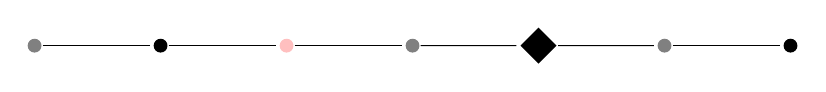
\begin{tikzpicture}[scale=0.8,->,>=stealth',shorten >=1pt,auto,node distance=3cm,
    thick,main node/.style={circle,draw,font=\footnotesize}, small node/.style={circle,font=\footnotesize,inner sep=0pt,minimum size=5pt}]   
    \begin{scope}%[xshift=10cm]
     \node[small node,fill=gray] (b) at (2,5) {};
      \node[small node,fill=black] (c) at (4,5) {};
      %\node[inner sep=0pt]  (d) at (6,5) {\includegraphics[width=.03\textwidth,right]{robot1.jpg}};
       \node[small node,fill=pink] (d) at (6,5) {};
       \node[small node,fill=gray] (e) at (8,5) {};    

      \node[diamond, fill=black]  (f) at (10,5) {};
      \node[small node,fill=gray] (i) at (12,5) {};
      \node[small node,fill=black] (j) at (14,5) {};
       \path[-,line width=0.3pt] (b) edge (c);
       \path[-,line width=0.3pt] (c) edge (d);
       \path[-,line width=0.3pt] (d) edge (e);
      \path[-,line width=0.3pt] (e) edge (f);
      \path[-,line width=0.3pt] (f) edge (i);
      \path[-,line width=0.3pt] (i) edge (j);
      %\path[-,line width=0.3pt, color=pink] (f) edge [bend left,-] (8.8,6.8);       

    \end{scope}
  \end{tikzpicture}
\end{frame}

%\begin{frame}{Compute} %%% CYCLE 2 %%%

\begin{frame}{Compute} %%% CYCLE 5 %%%

    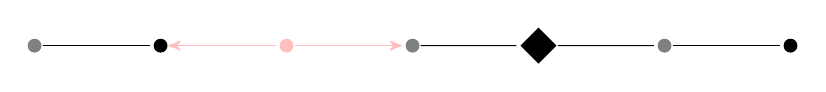
\begin{tikzpicture}[scale=0.8,->,>=stealth',shorten >=1pt,auto,node distance=3cm,
    thick,main node/.style={circle,draw,font=\footnotesize}, small node/.style={circle,font=\footnotesize,inner sep=0pt,minimum size=5pt}]   
    \begin{scope}%[xshift=10cm]
     \node[small node,fill=gray] (b) at (2,5) {};
      \node[small node,fill=black] (c) at (4,5) {};
      %\node[inner sep=0pt]  (d) at (6,5) {\includegraphics[width=.03\textwidth,right]{robot1.jpg}};
       \node[small node,fill=pink] (d) at (6,5) {};
       \node[small node,fill=gray] (e) at (8,5) {};    

      \node[diamond, fill=black]  (f) at (10,5) {};
      \node[small node,fill=gray] (i) at (12,5) {};
      \node[small node,fill=black] (j) at (14,5) {};
      \path[-,line width=0.3pt] (b) edge (c);
       \path[<-,line width=0.6pt, color=pink] (c) edge (d);
       \path[->,line width=0.6pt, color=pink] (d) edge (e);
      \path[-,line width=0.3pt] (e) edge (f);
      \path[-,line width=0.3pt] (f) edge (i);
      \path[-,line width=0.3pt] (i) edge (j);
      %\path[-,line width=0.3pt, color=pink] (f) edge [bend left,-] (8.8,6.8);       

    \end{scope}
  \end{tikzpicture}
\end{frame}


\begin{frame}{Move} %%% CYCLE 1 %%%

    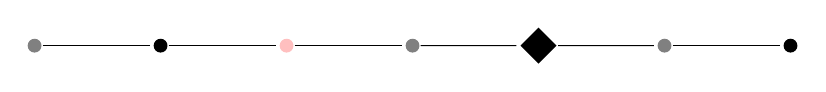
\begin{tikzpicture}[scale=0.8,->,>=stealth',shorten >=1pt,auto,node distance=3cm,
    thick,main node/.style={circle,draw,font=\footnotesize}, small node/.style={circle,font=\footnotesize,inner sep=0pt,minimum size=5pt}]   
    \begin{scope}%[xshift=10cm]
     \node[small node,fill=gray] (b) at (2,5) {};
      \node[small node,fill=black] (c) at (4,5) {};
      %\node[inner sep=0pt]  (d) at (6,5) {\includegraphics[width=.03\textwidth,right]{robot1.jpg}};
       \node[small node,fill=pink] (d) at (6,5) {};
       \node[small node,fill=gray] (e) at (8,5) {};    

      \node[diamond, fill=black]  (f) at (10,5) {};
      \node[small node,fill=gray] (i) at (12,5) {};
      \node[small node,fill=black] (j) at (14,5) {};
       \path[-,line width=0.3pt] (b) edge (c);
       \path[-,line width=0.3pt] (c) edge (d);
       \path[-,line width=0.3pt] (d) edge (e);
      \path[-,line width=0.3pt] (e) edge (f);
      \path[-,line width=0.3pt] (f) edge (i);
      \path[-,line width=0.3pt] (i) edge (j);
      %\path[-,line width=0.3pt, color=pink] (f) edge [bend left,-] (8.8,6.8);       

    \end{scope}
  \end{tikzpicture}
\end{frame}

\begin{frame}{Move} %%% CYCLE 3 %%%

    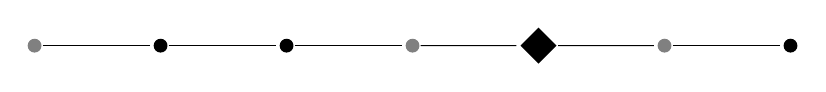
\begin{tikzpicture}[scale=0.8,->,>=stealth',shorten >=1pt,auto,node distance=3cm,
    thick,main node/.style={circle,draw,font=\footnotesize}, small node/.style={circle,font=\footnotesize,inner sep=0pt,minimum size=5pt}]   
    \begin{scope}%[xshift=10cm]
     \node[small node,fill=gray] (b) at (2,5) {};
      \node[small node,fill=black] (c) at (4,5) {};
      %\node[inner sep=0pt]  (d) at (6,5) {\includegraphics[width=.03\textwidth,right]{robot1.jpg}};
       \node[small node,fill=black] (d) at (6,5) {};
       \node[small node,fill=gray] (e) at (8,5) {};    

      \node[diamond, fill=black]  (f) at (10,5) {};
      \node[small node,fill=gray] (i) at (12,5) {};
      \node[small node,fill=black] (j) at (14,5) {};
       \path[-,line width=0.3pt] (b) edge (c);
       \path[-,line width=0.3pt] (c) edge (d);
       \path[-,line width=0.3pt] (d) edge (e);
      \path[-,line width=0.3pt] (e) edge (f);
      \path[-,line width=0.3pt] (f) edge (i);
      \path[-,line width=0.3pt] (i) edge (j);
      %\path[-,line width=0.3pt, color=pink] (f) edge [bend left,-] (8.8,6.8);       

    \end{scope}
  \end{tikzpicture}
\end{frame}

\begin{frame}{Look} %%% CYCLE 4 %%%

    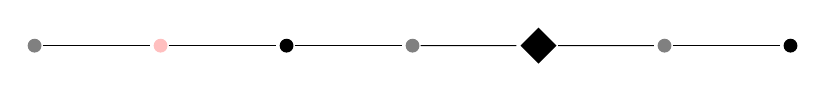
\begin{tikzpicture}[scale=0.8,->,>=stealth',shorten >=1pt,auto,node distance=3cm,
    thick,main node/.style={circle,draw,font=\footnotesize}, small node/.style={circle,font=\footnotesize,inner sep=0pt,minimum size=5pt}]   
    \begin{scope}%[xshift=10cm]
     \node[small node,fill=gray] (b) at (2,5) {};
      \node[small node,fill=pink] (c) at (4,5) {};
      %\node[inner sep=0pt]  (d) at (6,5) {\includegraphics[width=.03\textwidth,right]{robot1.jpg}};
       \node[small node,fill=black] (d) at (6,5) {};
       \node[small node,fill=gray] (e) at (8,5) {};    

      \node[diamond, fill=black]  (f) at (10,5) {};
      \node[small node,fill=gray] (i) at (12,5) {};
      \node[small node,fill=black] (j) at (14,5) {};
       \path[-,line width=0.3pt] (b) edge (c);
       \path[-,line width=0.3pt] (c) edge (d);
       \path[-,line width=0.3pt] (d) edge (e);
      \path[-,line width=0.3pt] (e) edge (f);
      \path[-,line width=0.3pt] (f) edge (i);
      \path[-,line width=0.3pt] (i) edge (j);
      %\path[-,line width=0.3pt, color=pink] (f) edge [bend left,-] (8.8,6.8);       

    \end{scope}
  \end{tikzpicture}
\end{frame}

\begin{frame}{Compute} %%% CYCLE 5 %%%

    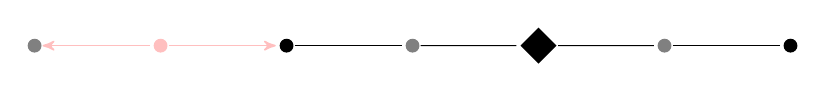
\begin{tikzpicture}[scale=0.8,->,>=stealth',shorten >=1pt,auto,node distance=3cm,
    thick,main node/.style={circle,draw,font=\footnotesize}, small node/.style={circle,font=\footnotesize,inner sep=0pt,minimum size=5pt}]   
    \begin{scope}%[xshift=10cm]
     \node[small node,fill=gray] (b) at (2,5) {};
      \node[small node,fill=pink] (c) at (4,5) {};
      %\node[inner sep=0pt]  (d) at (6,5) {\includegraphics[width=.03\textwidth,right]{robot1.jpg}};
       \node[small node,fill=black] (d) at (6,5) {};
       \node[small node,fill=gray] (e) at (8,5) {};    

      \node[diamond, fill=black]  (f) at (10,5) {};
      \node[small node,fill=gray] (i) at (12,5) {};
      \node[small node,fill=black] (j) at (14,5) {};
       \path[<-,line width=0.6pt, color=pink] (b) edge (c);
       \path[->,line width=0.6pt, color=pink] (c) edge (d);
       \path[-,line width=0.3pt]  (d) edge (e);
      \path[-,line width=0.3pt] (e) edge (f);
      \path[-,line width=0.3pt] (f) edge (i);
      \path[-,line width=0.3pt] (i) edge (j);
      %\path[-,line width=0.3pt, color=pink] (f) edge [bend left,-] (8.8,6.8);       

    \end{scope}
  \end{tikzpicture}
\end{frame}

\begin{frame}{Move} %%% CYCLE 6 %%%

    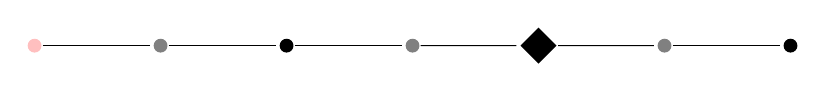
\begin{tikzpicture}[scale=0.8,->,>=stealth',shorten >=1pt,auto,node distance=3cm,
    thick,main node/.style={circle,draw,font=\footnotesize}, small node/.style={circle,font=\footnotesize,inner sep=0pt,minimum size=5pt}]   
    \begin{scope}%[xshift=10cm]
     \node[small node,fill=pink] (b) at (2,5) {};
      \node[small node,fill=gray] (c) at (4,5) {};
      %\node[inner sep=0pt]  (d) at (6,5) {\includegraphics[width=.03\textwidth,right]{robot1.jpg}};
       \node[small node,fill=black] (d) at (6,5) {};
       \node[small node,fill=gray] (e) at (8,5) {};    

      \node[diamond, fill=black]  (f) at (10,5) {};
      \node[small node,fill=gray] (i) at (12,5) {};
      \node[small node,fill=black] (j) at (14,5) {};
       \path[-,line width=0.3pt] (b) edge (c);
       \path[-,line width=0.3pt] (c) edge (d);
       \path[-,line width=0.3pt] (d) edge (e);
      \path[-,line width=0.3pt] (e) edge (f);
      \path[-,line width=0.3pt] (f) edge (i);
      \path[-,line width=0.3pt] (i) edge (j);
      %\path[-,line width=0.3pt, color=pink] (f) edge [bend left,-] (8.8,6.8);       

    \end{scope}
  \end{tikzpicture}
\end{frame}

\begin{frame}{Move} %%% CYCLE 7 %%%

    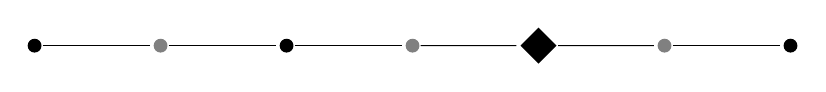
\begin{tikzpicture}[scale=0.8,->,>=stealth',shorten >=1pt,auto,node distance=3cm,
    thick,main node/.style={circle,draw,font=\footnotesize}, small node/.style={circle,font=\footnotesize,inner sep=0pt,minimum size=5pt}]   
    \begin{scope}%[xshift=10cm]
     \node[small node,fill=black] (b) at (2,5) {};
      \node[small node,fill=gray] (c) at (4,5) {};
      %\node[inner sep=0pt]  (d) at (6,5) {\includegraphics[width=.03\textwidth,right]{robot1.jpg}};
       \node[small node,fill=black] (d) at (6,5) {};
       \node[small node,fill=gray] (e) at (8,5) {};    

      \node[diamond, fill=black]  (f) at (10,5) {};
      \node[small node,fill=gray] (i) at (12,5) {};
      \node[small node,fill=black] (j) at (14,5) {};
       \path[-,line width=0.3pt] (b) edge (c);
       \path[-,line width=0.3pt] (c) edge (d);
       \path[-,line width=0.3pt] (d) edge (e);
      \path[-,line width=0.3pt] (e) edge (f);
      \path[-,line width=0.3pt] (f) edge (i);
      \path[-,line width=0.3pt] (i) edge (j);
      %\path[-,line width=0.3pt, color=pink] (f) edge [bend left,-] (8.8,6.8);       

    \end{scope}
  \end{tikzpicture}
\end{frame}

\begin{frame}{Robots: Asynchronous} %%% CYCLE 7 %%%

    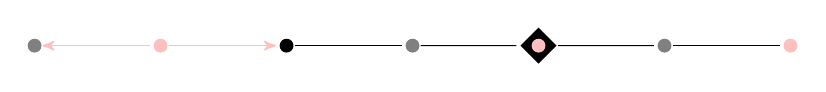
\begin{tikzpicture}[scale=0.8,->,>=stealth',shorten >=1pt,auto,node distance=3cm,
    thick,main node/.style={circle,draw,font=\footnotesize}, small node/.style={circle,font=\footnotesize,inner sep=0pt,minimum size=5pt}]   
   \begin{scope}%[xshift=10cm]
     \node[small node,fill=gray] (b) at (2,5) {};
      \node[small node,fill=pink] (c) at (4,5) {};
      %\node[inner sep=0pt]  (d) at (6,5) {\includegraphics[width=.03\textwidth,right]{robot1.jpg}};
       \node[small node,fill=black] (d) at (6,5) {};
       \node[small node,fill=gray] (e) at (8,5) {};    

      \node[diamond, fill=black]  (f) at (10,5) {};
      \node[small node,fill=pink]  at (10,5) {};
      \node[small node,fill=gray] (i) at (12,5) {};
      \node[small node,fill=pink] (j) at (14,5) {};
       \path[<-,line width=0.6pt, color=pink] (b) edge (c);
       \path[->,line width=0.6pt, color=pink] (c) edge (d);
       \path[-,line width=0.3pt]  (d) edge (e);
      \path[-,line width=0.3pt] (e) edge (f);
      \path[-,line width=0.3pt] (f) edge (i);
      \path[-,line width=0.3pt] (i) edge (j);
      %\path[-,line width=0.3pt, color=pink] (f) edge [bend left,-] (8.8,6.8);       

    \end{scope}
  \end{tikzpicture}
\end{frame}

\begin{frame}{Robots: Asynchronous} %%% CYCLE 7 %%%

    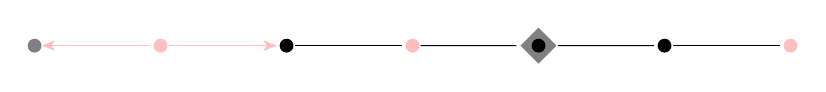
\begin{tikzpicture}[scale=0.8,->,>=stealth',shorten >=1pt,auto,node distance=3cm,
    thick,main node/.style={circle,draw,font=\footnotesize}, small node/.style={circle,font=\footnotesize,inner sep=0pt,minimum size=5pt}]   
   \begin{scope}%[xshift=10cm]
     \node[small node,fill=gray] (b) at (2,5) {};
      \node[small node,fill=pink] (c) at (4,5) {};
      %\node[inner sep=0pt]  (d) at (6,5) {\includegraphics[width=.03\textwidth,right]{robot1.jpg}};
       \node[small node,fill=black] (d) at (6,5) {};
       \node[small node,fill=pink] (e) at (8,5) {};  
       
      \node[diamond, fill=gray]  (f)  at (10,5) {};
      \node[small node,fill=black]   at (10,5) {};
      %\node[small node,fill=pink]  at (10,5) {};
      \node[small node,fill=black] (i) at (12,5) {};
      \node[small node,fill=pink] (j) at (14,5) {};
       \path[<-,line width=0.6pt, color=pink] (b) edge (c);
       \path[->,line width=0.6pt, color=pink] (c) edge (d);
       \path[-,line width=0.3pt]  (d) edge (e);
      \path[-,line width=0.3pt] (e) edge (f);
      \path[-,line width=0.3pt] (f) edge (i);
      \path[-,line width=0.3pt] (i) edge (j);
      %\path[-,line width=0.3pt, color=pink] (f) edge [bend left,-] (8.8,6.8);       

    \end{scope}
  \end{tikzpicture}
\end{frame}

\begin{frame}{Robots: Asynchronous} %%% CYCLE 7 %%%

    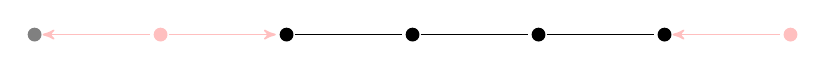
\begin{tikzpicture}[scale=0.8,->,>=stealth',shorten >=1pt,auto,node distance=3cm,
    thick,main node/.style={circle,draw,font=\footnotesize}, small node/.style={circle,font=\footnotesize,inner sep=0pt,minimum size=5pt}]   
   \begin{scope}%[xshift=10cm]
     \node[small node,fill=gray] (b) at (2,5) {};
      \node[small node,fill=pink] (c) at (4,5) {};
      %\node[inner sep=0pt]  (d) at (6,5) {\includegraphics[width=.03\textwidth,right]{robot1.jpg}};
       \node[small node,fill=black] (d) at (6,5) {};
       \node[small node,fill=black] (e) at (8,5) {};    

      \node[small node,fill=black]  (f) at (10,5) {};
      %\node[small node,fill=pink]  at (10,5) {};
      \node[small node,fill=black] (i) at (12,5) {};
      \node[small node,fill=pink] (j) at (14,5) {};
       \path[<-,line width=0.6pt, color=pink] (b) edge (c);
       \path[->,line width=0.6pt, color=pink] (c) edge (d);
       \path[-,line width=0.3pt]  (d) edge (e);
      \path[-,line width=0.3pt] (e) edge (f);
      \path[-,line width=0.3pt] (f) edge (i);
      \path[<-,line width=0.6pt, color=pink] (i) edge (j);
      %\path[-,line width=0.3pt, color=pink] (f) edge [bend left,-] (8.8,6.8);       

    \end{scope}
  \end{tikzpicture}
\end{frame}

\begin{frame}{Robots: Oblivious} %%% CYCLE 7 %%%

    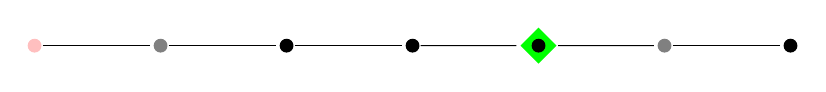
\begin{tikzpicture}[scale=0.8,->,>=stealth',shorten >=1pt,auto,node distance=3cm,
    thick,main node/.style={circle,draw,font=\footnotesize}, small node/.style={circle,font=\footnotesize,inner sep=0pt,minimum size=5pt}]   
   \begin{scope}%[xshift=10cm]
     \node[small node,fill=pink] (b) at (2,5) {};
      \node[small node,fill=gray] (c) at (4,5) {};
      %\node[inner sep=0pt]  (d) at (6,5) {\includegraphics[width=.03\textwidth,right]{robot1.jpg}};
       \node[small node,fill=black] (d) at (6,5) {};
       \node[small node,fill=black] (e) at (8,5) {};    

      \node[diamond, fill=green]  (f) at (10,5) {};
      \node[small node,fill=black]  at (10,5) {};
      \node[small node,fill=gray] (i) at (12,5) {};
      \node[small node,fill=black] (j) at (14,5) {};
       \path[-,line width=0.3pt] (b) edge (c);
       \path[-,line width=0.3pt] (c) edge (d);
       \path[-,line width=0.3pt]  (d) edge (e);
      \path[-,line width=0.3pt] (e) edge (f);
      \path[-,line width=0.3pt] (f) edge (i);
      \path[-,line width=0.3pt] (i) edge (j);
      %\path[-,line width=0.3pt, color=pink] (f) edge [bend left,-] (8.8,6.8);       

    \end{scope}
  \end{tikzpicture}
\end{frame}

%%%%%%%%%%%%%%%%%%%%%%%%%%%%%%%%%%%%%%%%%%%%%%%%%%%%%%
%%%%%%%%%%%%%%%%%%%%%%%%%%%%%%%%%%%%%%%%%%%%%%%%%%%%%%
\section{\scshape Problem}
\subsection{frame 1}
\begin{frame}{Exploration with termination}
\begin{itemize}
 \item initial configuration with no towers
 \item \textcolor{gray}{all nodes must be visited}
 \item \textcolor{gray}{after finite time robots should stay idle}
\end{itemize}

\end{frame}

\begin{frame}{Exploration with termination}
\begin{itemize}
 \item \textcolor{gray}{initial configuration with no towers}
 \item all nodes must be visited
 \item \textcolor{gray}{after finite time robots should stay idle}
\end{itemize}

\end{frame}

\begin{frame}{Exploration with termination}
\begin{itemize}
 \item \textcolor{gray}{initial configuration with no towers}
 \item \textcolor{gray}{all nodes must be visited}
 \item after finite time robots should stay idle
\end{itemize}

\end{frame}
%
%
%%%%%%%%%%%%%%%%%%%%%%%%%%%%%%%%%%%%%%%%%%%%%%%%%%%%%%%
%%%%%%%%%%%%%%%%%%%%%%%%%%%%%%%%%%%%%%%%%%%%%%%%%%%%%%%
%\subsection{frame 1}
%\begin{frame}{frame 1}
%
%\end{frame}
%
%%%%%%%%%%%%%%%%%%%%%%%%%%%%%%%%%%%%%%%%%%%%%%%%%%%%%%
%%%%%%%%%%%%%%%%%%%%%%%%%%%%%%%%%%%%%%%%%%%%%%%%%%%%%%
\section{\scshape Results}
\subsection{Frame 1}
\begin{frame}{Frame 1}

\end{frame}

\end{document}
